\usepackage{fullpage}
\RequirePackage[l2tabu, orthodox]{nag}
\usepackage[british]{babel}
\usepackage[toc,page]{appendix}
\usepackage[T1]{fontenc}
\usepackage{amsmath}
\usepackage{amssymb}
\usepackage[T1]{fontenc}
%\usepackage{natbib}
%\setcitestyle{square}
\usepackage[utf8]{inputenc}
\usepackage{amsthm}
\usepackage{color}
\usepackage{float}
\usepackage{authblk}
%\usepackage{todonotes}
\usepackage{algorithmicx}
\usepackage{algpseudocode}% http://ctan.org/pkg/algorithmicx
\usepackage{microtype}
\usepackage{caption}
\usepackage{dsfont}
\usepackage{svg}
\DeclareCaptionFont{white}{\color{white}}
\DeclareCaptionFormat{listing}{\colorbox{gray}{\parbox{\textwidth}{#1#2#3}}}
\captionsetup[lstlisting]{format=listing,labelfont=white,textfont=white}

\usepackage{cooltooltips}
\usepackage{graphicx}
\usepackage{color}
\usepackage{hyperref}
\usepackage{centernot}



\usepackage{alltt}
\usepackage{listings}
\usepackage{algorithm}
%\usepackage{algorithmicx}
\usepackage{subfig}
\lstset{% parameters for all code listings
language=Python,
frame=single,
basicstyle=\small, % nothing smaller than \footnotesize, please
tabsize=2,
numbers=left,
% framexleftmargin=2em, % extend frame to include line numbers
%xrightmargin=2em, % extra space to fit 79 characters
breaklines=true,
breakatwhitespace=true,
prebreak={/},
captionpos=b,
columns=fullflexible,
escapeinside={\#*}{\^^M}
}

\usepackage{todonotes}

\usepackage{tikz}
\usetikzlibrary{arrows}
\usetikzlibrary{automata,positioning}
\usepackage{forest}

\newcommand{\abpsender}[1][]{
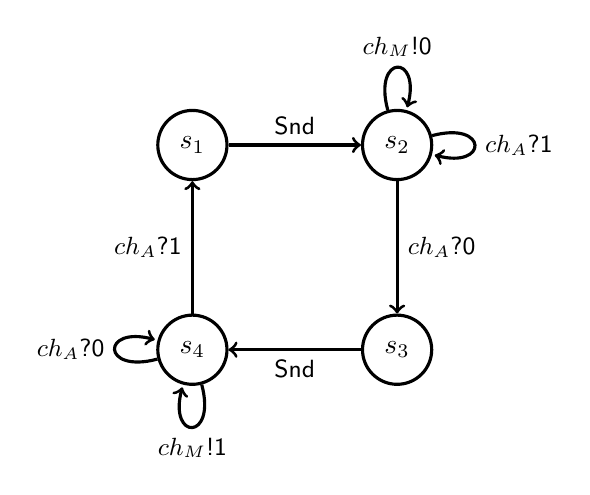
\begin{tikzpicture} [->,auto,node distance=2.6cm,line width=0.4mm]
  \node[state] (1) {$s_1$};
  \node[state] (2) [right of=1] {$s_2$};
  \node[state] (3) [below of=2] {$s_3$};
  \node[state] (4) [left of=3] {$s_4$};

  \path[every node/.style={font=\sffamily\small}]
    (1) edge node [above] {Snd} (2)
    (2) edge node [right] {$ch_A$?0} (3)
        edge [loop right] node {$ch_A$?1} (2)
        edge [loop above] node {$ch_M$!0} (2)
    (3) edge node [below] {Snd} (4)
    (4) edge node [left] {$ch_A$?1} (1)
        edge [loop left] node {$ch_A$?0} (4)
        edge [loop below] node {$ch_M$!1} (4);
\end{tikzpicture}
}

\newcommand{\abpreceiver}[1][]{
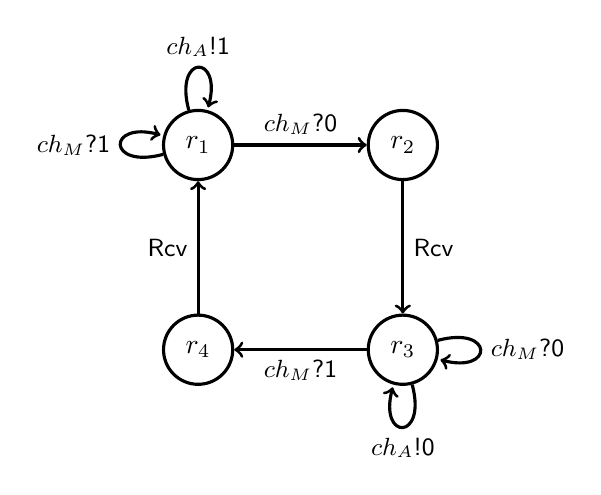
\begin{tikzpicture} [->,auto,node distance=2.6cm,line width=0.4mm]

  \node[state] (1) {$r_1$};
  \node[state] (2) [right of=1] {$r_2$};
  \node[state] (3) [below of=2] {$r_3$};
  \node[state] (4) [left of=3] {$r_4$};

  \path[every node/.style={font=\sffamily\small}]
    (1) edge node [above] {$ch_M$?0} (2)
        edge [loop left] node {$ch_M$?1} (1)
        edge [loop above] node {$ch_A$!1} (1)
    (2) edge node [right] {Rcv} (3)
    (3) edge node [below] {$ch_M$?1} (4)
        edge [loop right] node {$ch_M$?0} (3)
        edge [loop below] node {$ch_A$!0} (3)
    (4) edge node [left] {Rcv} (1);

\end{tikzpicture}
}


\newcommand{\swsender}[1][]{
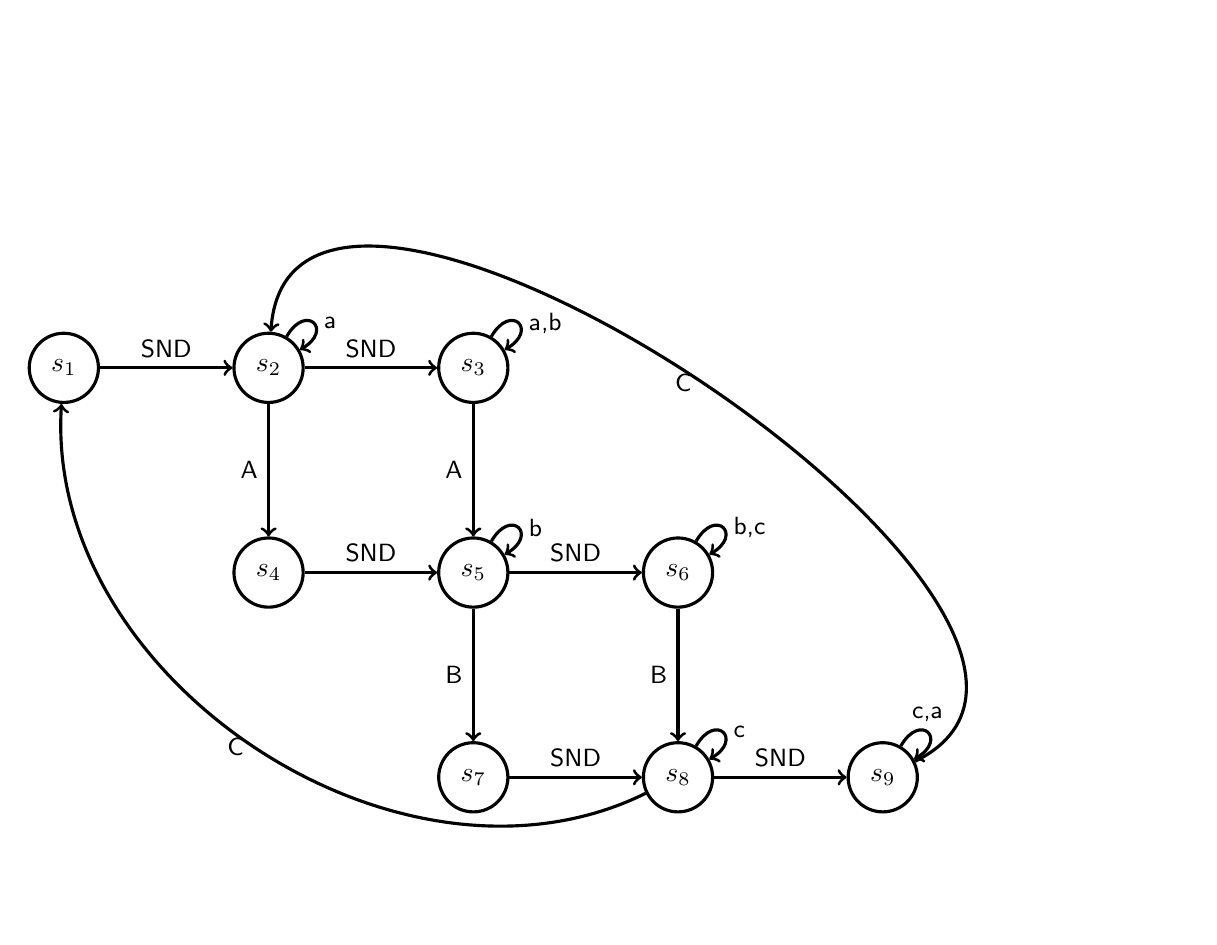
\begin{tikzpicture} [->,auto,node distance=2.6cm,line width=0.4mm]
  \node[state] (1) {$s_1$};
  \node[state] (2) [right of=1] {$s_2$};
  \node[state] (3) [right of=2] {$s_3$};
  \node[state] (4) [below of=2] {$s_4$};
  \node[state] (5) [below of=3] {$s_5$};
  \node[state] (6) [right of=5] {$s_6$};
  \node[state] (7) [below of=5] {$s_7$};
  \node[state] (8) [below of=6] {$s_8$};
  \node[state] (9) [right of=8] {$s_9$};

  \path[->,every loop/.style={in=30, out=60, looseness=3}, every node/.style={font=\sffamily\small}]
    (1) edge node [above] {SND} (2)
    (2) edge node [above] {SND} (3)
        edge [loop right] node {a} (2)
        edge node [left] {A} (4)
    (3) edge node [left] {A} (5)
        edge [loop right] node {a,b} (3)
    (4) edge node [above] {SND} (5)
    (5) edge node [above] {SND} (6)
        edge [loop right] node {b} (5)
        edge node [left] {B} (7)
    (6) edge node [left] {B} (8)
        edge [loop right] node {b,c} (6)
    (7) edge node [above] {SND} (8)
    (8) edge node [above] {SND} (9)
        edge [loop right] node {c} (8)
        edge [bend left=60] node [left] {C} (1)
    (9) edge [bend right=120] node [left] {C} (2)
        edge [loop above] node {c,a} (9);




\end{tikzpicture}
}

\newcommand{\swreceiver}[1][]{
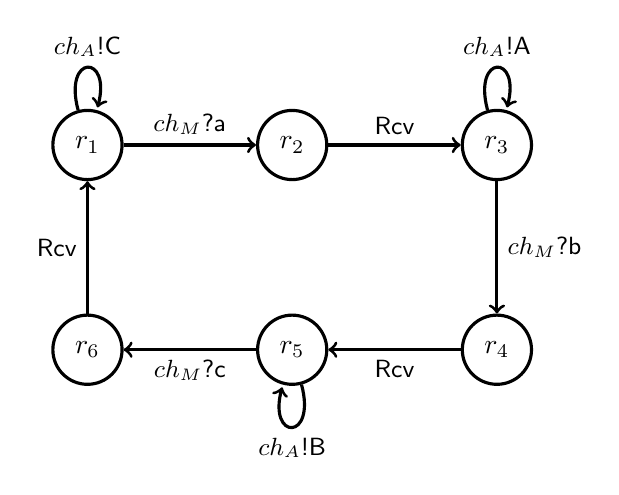
\begin{tikzpicture} [->,auto,node distance=2.6cm,line width=0.4mm]

  \node[state] (1) {$r_1$};
  \node[state] (2) [right of=1] {$r_2$};
  \node[state] (3) [right of=2] {$r_3$};
  \node[state] (4) [below of=3] {$r_4$};
  \node[state] (5) [left of=4] {$r_5$};
  \node[state] (6) [left of=5] {$r_6$};

  \path[every node/.style={font=\sffamily\small}]
    (1) edge node [above] {$ch_M$?a} (2)
  edge [loop above] node {$ch_A$!C} (1)
    (2) edge node [above] {Rcv} (3)
    (3) edge node [right] {$ch_M$?b} (4)
  edge [loop above] node {$ch_A$!A} (3)
    (4) edge node [below] {Rcv} (5)
    (5) edge node [below] {$ch_M$?c} (6)
  edge [loop below] node {$ch_A$!B} (5)
    (6) edge node [left] {Rcv} (1);

\end{tikzpicture}
}


\newcommand{\swobserver}[1][]{
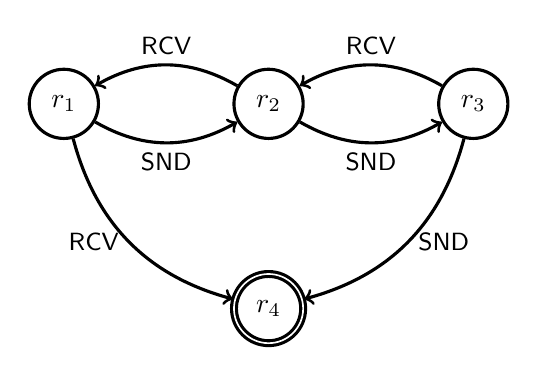
\begin{tikzpicture} [->,auto,node distance=2.6cm,line width=0.4mm]

  \node[state] (1) {$r_1$};
  \node[state] (2) [right of=1] {$r_2$};
  \node[state] (3) [right of=2] {$r_3$};
  \node[state,accepting] (4) [below of=2] {$r_4$};


  \path[every node/.style={font=\sffamily\small}]
    (1) edge [bend right] node [below] {SND} (2)
  edge [bend right] node [left] {RCV} (4)
    (2) edge [bend right] node [below] {SND} (3)
  edge [bend right] node [above] {RCV} (1)
    (3) edge [bend left] node [right] {SND} (4)
  edge [bend right] node [above] {RCV} (2);

\end{tikzpicture}
}



\newcommand{\abpobserver}[1][]{
\begin{tikzpicture} [->,auto,node distance=2.6cm,line width=0.4mm]

%\begin{tikzpicture}[->,>=stealth',shorten >=1pt,auto,node distance=3cm,
%  thick,main node/.style={circle,fill=blue!20,draw,font=\sffamily\Large\bfseries}]

  \node[state] (1) {$o_1$};
  \node[state,accepting] (3) [right of=1] {$o_2$};
  \node[state] (2) [right of=2] {$o_3$};

  \path[every node/.style={font=\sffamily\small}]
    (1) edge [bend left] node [above] {Snd} (2)
        edge node [above] {Rcv} (3)
    (2) edge [bend left] node [below] {Rcv} (1)
        edge node [above] {Snd} (3);
\end{tikzpicture}
}

% Alter some LaTeX defaults for better treatment of figures:
    % See p.105 of "TeX Unbound" for suggested values.
    % See pp. 199-200 of Lamport's "LaTeX" book for details.
    % General parameters, for ALL pages:
    \renewcommand{\topfraction}{0.9}	% max fraction of floats at top
    \renewcommand{\bottomfraction}{0.8}	% max fraction of floats at bottom
    % Parameters for TEXT pages (not float pages):
    \setcounter{topnumber}{2}
    \setcounter{bottomnumber}{2}
    \setcounter{totalnumber}{4} % 2 may work better
    \setcounter{dbltopnumber}{2} % for 2-column pages
    \renewcommand{\dbltopfraction}{0.9}	% fit big float above 2-col. text
    \renewcommand{\textfraction}{0.07}	% allow minimal text w. figs
    % Parameters for FLOAT pages (not text pages):
    \renewcommand{\floatpagefraction}{0.7}	% require fuller float pages
% N.B.: floatpagefraction MUST be less than topfraction !!
    \renewcommand{\dblfloatpagefraction}{0.7}	% require fuller float pages

% remember to use [htp] or [htpb] for placement

\theoremstyle{plain}
\newtheorem{thm}{Theorem}[section] % reset theorem numbering for each chapter
\theoremstyle{definition}
\newtheorem{defn}[thm]{Definition} % definition numbers are dependent on theorem numbers
\newtheorem{theorem}[thm]{Theorem}
\newtheorem{lemma}[thm]{Lemma}
\newtheorem{exmp}{Example}[section]

\usepackage{fancyvrb}
%\DefineVerbatimEnvironment{code}{Verbatim}{fontsize=\small
%\DefineVerbatimEnvironment{example}{Verbatim}{fontsize=\small}

\usepackage{url}
\urldef{\mailsa}\path|josh0151@student.uu.se |
\urldef{\mailsb}\path|bjfo5755@student.uu.se |
\newcommand{\keywords}[1]{\par\addvspace\baselineskip
\noindent\keywordname\enspace\ignorespaces#1}


\usepackage{tikz} \usetikzlibrary{trees}
\usepackage{hyperref} % should always be the last package

% useful colours (use sparingly!):
\newcommand{\blue}[1]{{\color{blue}#1}}
\newcommand{\green}[1]{{\color{green}#1}}
\newcommand{\red}[1]{{\color{red}#1}}

% useful wrappers for algorithmic/Python notation:
\newcommand{\length}[1]{\text{len}(#1)}
\newcommand{\twodots}{\mathinner{\ldotp\ldotp}} % taken from clrscode3e.sty
\newcommand{\Oh}[1]{\mathcal{O}\left(#1\right)}

% useful (wrappers for) math symbols:
\newcommand{\Cardinality}[1]{\left\lvert#1\right\rvert}
%\newcommand{\Cardinality}[1]{\##1}
\newcommand{\Ceiling}[1]{\left\lceil#1\right\rceil}
\newcommand{\Floor}[1]{\left\lfloor#1\right\rfloor}
\newcommand{\Iff}{\Leftrightarrow}
\newcommand{\Implies}{\Rightarrow}
\newcommand{\Intersect}{\cap}
\newcommand{\Sequence}[1]{\left[#1\right]}
\newcommand{\Set}[1]{\left\{#1\right\}}
\newcommand{\SetComp}[2]{\Set{#1\SuchThat#2}}
\newcommand{\SuchThat}{\mid}
\newcommand{\Tuple}[1]{\langle#1\rangle}
\newcommand{\Union}{\cup}
\newcommand{\conf}[1]{(#1)}
\newcommand{\trans}[3]{#1 \xrightarrow{#2} #3}
\newcommand{\subword}{\sqsubseteq}
\newcommand{\e}[1]{\emph{#1}}
\usetikzlibrary{positioning,shapes,shadows,arrows}

\usepackage{url}
\usepackage{tabularx}

\usepackage{booktabs,array}
\def\Midrule{\midrule[\heavyrulewidth]}
\newcount\rowc

\makeatletter
\def\ttabular{%
\hbox\bgroup
\let\\\cr
\valign\bgroup
\global\rowc\@ne
\hbox to 12em{\strut \hfill##\hfill}%
&&%
\global\advance\rowc\@ne
\hbox to 12em{\strut\hfill##\hfill}%
\cr}
\def\endttabular{%
\crcr\egroup\egroup}

\makeatletter
\def\ttabulartwo{%
\hbox\bgroup
\let\\\cr
\valign\bgroup
\global\rowc\@ne
\hbox to 7em{\strut \hfill##\hfill}%
&&%
\global\advance\rowc\@ne
\hbox to 7em{\strut\hfill##\hfill}%
\cr}
\def\endttabulartwo{%
\crcr\egroup\egroup}


\usepackage{amsthm}


\tikzset{
  graph vertex/.style={
    circle,
    draw,
  },
  graph directed edge/.style={
    ->,
    >=stealth,
    thick,
  },
  graph tree edge/.style={
    graph directed edge
  },
  graph forward edge/.style={
    graph directed edge,
    every edge/.style={
      edge node={node [fill=white,font=\scriptsize] {f}},
      loosely dotted,
      draw,
    },
  },
  graph back edge/.style={
    graph directed edge,
    every edge/.style={
      edge node={node [fill=white,font=\scriptsize] {b}},
      densely dotted,
      draw,
    },
  },
  graph cross edge/.style={
    graph directed edge,
    every edge/.style={
      dotted,
      draw,
    },
  },
}

\newcommand{\abstraction}[1][]{
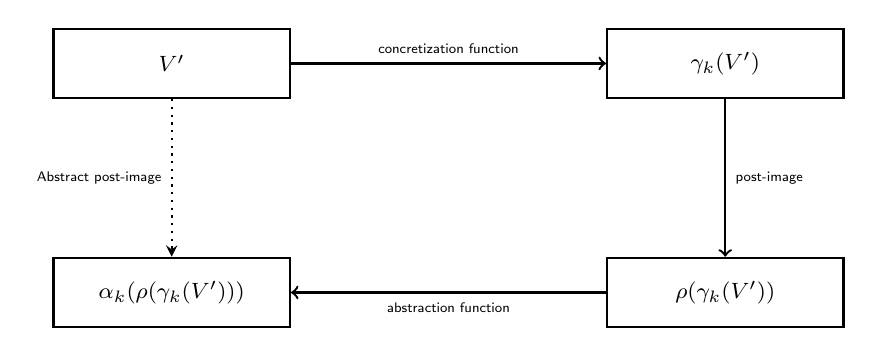
\begin{tikzpicture} [->,auto,node distance=2cm and 4cm,line width=0.3mm, font=\footnotesize]

  \node[state] (1) [rectangle, minimum width=3cm] {$V'$};
  \node[state] (2) [rectangle, minimum width=3cm,right=of 1] {$\gamma_k(V')$};
  \node[state] (3) [rectangle, minimum width=3cm,below=of 2] {$\rho(\gamma_k(V'))$};
  \node[state] (4) [rectangle, minimum width=3cm,left=of 3] {$\alpha_k(\rho(\gamma_k(V')))$};

  \path[every node/.style={font=\sffamily\tiny}]
    (1) edge node [above] {concretization function} (2)
    (2) edge node [right] {post-image} (3)
    (3) edge node [below] {abstraction function} (4);
  \path[graph cross edge, every node/.style={font=\sffamily\tiny}]
    (1) edge node [left] {Abstract post-image} (4);

\end{tikzpicture}
}
